\documentclass[11pt]{article}
\usepackage[utf8]{inputenc}
\usepackage{amsmath}
\usepackage{amssymb}
\usepackage{listings}
\usepackage{xcolor}
\usepackage{tikz}
\usepackage{hyperref}
\usepackage{geometry}
\usepackage{graphicx}
\usepackage{colortbl}
\usepackage{algorithm}
\usepackage{algpseudocode}

\geometry{a4paper, margin=1in}

% Code style settings
\lstset{
    language=C++,
    basicstyle=\ttfamily\small,
    keywordstyle=\color{blue},
    commentstyle=\color{green!60!black},
    stringstyle=\color{red},
    numbers=left,
    numberstyle=\tiny\color{gray},
    breaklines=true,
    frame=single,
    backgroundcolor=\color{gray!10}
}

% TikZ settings
\usetikzlibrary{shapes, arrows, positioning}

\title{ALE Implementation Headers Documentation}
\author{gsIncompressibleFlow Module}
\date{\today}

\begin{document}

\maketitle
\tableofcontents
\newpage

\section{Overview}

This document provides a detailed description of the core header files for the ALE (Arbitrary Lagrangian-Eulerian) implementation in the gsIncompressibleFlow module.

\section{Mathematical Formulation}

\subsection{ALE Framework}

The ALE method combines the advantages of Lagrangian and Eulerian descriptions. In the ALE framework, the computational mesh can move arbitrarily, independent of the fluid motion. The key concept is the introduction of a reference configuration $\hat{\Omega}$ that maps to the current configuration $\Omega_t$ through:

\begin{equation}
\mathcal{A}_t: \hat{\Omega} \rightarrow \Omega_t, \quad \hat{x} \mapsto x = \mathcal{A}_t(\hat{x})
\end{equation}

The mesh velocity is defined as:
\begin{equation}
w = \frac{\partial \mathcal{A}_t}{\partial t}\bigg|_{\hat{x}}
\end{equation}

\subsection{Incompressible Navier-Stokes Equations in ALE Form}

The incompressible Navier-Stokes equations in ALE form are:

\begin{align}
\rho\left(\frac{\partial u}{\partial t}\bigg|_{\hat{x}} + (u - w) \cdot \nabla u\right) - \nabla \cdot \sigma &= f \quad \text{in } \Omega_t \\
\nabla \cdot u &= 0 \quad \text{in } \Omega_t
\end{align}

where:
\begin{itemize}
    \item $u$ is the fluid velocity
    \item $w$ is the mesh velocity
    \item $\sigma = -pI + 2\mu\varepsilon(u)$ is the stress tensor
    \item $\varepsilon(u) = \frac{1}{2}(\nabla u + \nabla u^T)$ is the strain rate tensor
    \item $\rho$ is the fluid density
    \item $\mu$ is the dynamic viscosity
    \item $p$ is the pressure
    \item $f$ is the body force
\end{itemize}

\subsection{Weak Formulation}

Multiplying by test functions $(v, q) \in V \times Q$ and integrating by parts:

\begin{align}
\int_{\Omega_t} \rho\frac{\partial u}{\partial t}\bigg|_{\hat{x}} \cdot v \, d\Omega + \int_{\Omega_t} \rho(u - w) \cdot \nabla u \cdot v \, d\Omega &\\
+ \int_{\Omega_t} 2\mu\varepsilon(u) : \varepsilon(v) \, d\Omega - \int_{\Omega_t} p \nabla \cdot v \, d\Omega &= \int_{\Omega_t} f \cdot v \, d\Omega \\
\int_{\Omega_t} q \nabla \cdot u \, d\Omega &= 0
\end{align}

The key ALE contribution is the convective term:
\begin{equation}
\boxed{\int_{\Omega_t} \rho(u - w) \cdot \nabla u \cdot v \, d\Omega}
\end{equation}

\subsection{Time Discretization}

Using implicit Euler (first-order backward difference) for time discretization:

\begin{equation}
\frac{\partial u}{\partial t}\bigg|_{\hat{x}}^{n+1} \approx \frac{u^{n+1} - u^n}{\Delta t}
\end{equation}

For the mesh velocity, we use:
\begin{equation}
w^{n+1} = \frac{x^{n+1} - x^n}{\Delta t} = \frac{d^{n+1} - d^n}{\Delta t}
\end{equation}

where $d$ represents the mesh displacement from the reference configuration.

\subsection{Discretized Weak Form}

The fully discretized weak form at time step $n+1$ becomes:

\begin{align}
\int_{\Omega_{n+1}} \rho\frac{u^{n+1} - u^n}{\Delta t} \cdot v \, d\Omega + \int_{\Omega_{n+1}} \rho(u^{n+1} - w^{n+1}) \cdot \nabla u^{n+1} \cdot v \, d\Omega &\\
+ \int_{\Omega_{n+1}} 2\mu\varepsilon(u^{n+1}) : \varepsilon(v) \, d\Omega - \int_{\Omega_{n+1}} p^{n+1} \nabla \cdot v \, d\Omega &= \int_{\Omega_{n+1}} f^{n+1} \cdot v \, d\Omega \\
\int_{\Omega_{n+1}} q \nabla \cdot u^{n+1} \, d\Omega &= 0
\end{align}

\subsection{Matrix Form}

After spatial discretization using finite elements, the system can be written in matrix form:

\begin{equation}
\begin{bmatrix}
\frac{1}{\Delta t}M + A(u^{n+1}) + K & B^T \\
B & 0
\end{bmatrix}
\begin{bmatrix}
u^{n+1} \\
p^{n+1}
\end{bmatrix}
=
\begin{bmatrix}
F + \frac{1}{\Delta t}M u^n + A_{ALE}(w^{n+1}) \\
0
\end{bmatrix}
\end{equation}

where:
\begin{itemize}
    \item $M$ is the mass matrix
    \item $K$ is the stiffness matrix (viscous term)
    \item $A(u)$ is the convection matrix
    \item $A_{ALE}(w)$ represents the ALE correction to convection
    \item $B$ is the divergence matrix
    \item $F$ includes body forces and boundary conditions
\end{itemize}

\subsection{ALE Convection Term Implementation}

The ALE convection term is implemented as:

\begin{equation}
[A_{ALE}]_{ij} = \int_{\Omega} \rho \varphi_i \cdot ((u - w) \cdot \nabla \varphi_j) \, d\Omega
\end{equation}

where $\varphi_i$ and $\varphi_j$ are the finite element basis functions. The implementation computes:

\begin{enumerate}
    \item Relative velocity: $u_{rel} = u - w$
    \item Gradient in physical space: $\nabla \varphi_j = J^{-T} \nabla_{\xi} \varphi_j$
    \item Integration: $\sum_{q} w_q \, \varphi_i(x_q) \cdot (u_{rel}(x_q) \cdot \nabla \varphi_j(x_q)) \, |J|$
\end{enumerate}

where $J$ is the Jacobian of the geometric mapping, $x_q$ are quadrature points, and $w_q$ are quadrature weights.

\subsection{Geometric Conservation Law (GCL)}

For maintaining consistency, the discrete GCL should be satisfied:

\begin{equation}
\frac{\partial J}{\partial t} - \nabla \cdot (J w) = 0
\end{equation}

This ensures that constant solutions remain constant on moving meshes. In our implementation, this is implicitly satisfied through consistent mesh velocity computation.

\subsection{Mesh Motion Strategies}

The implementation supports various mesh motion strategies:

\subsubsection{Prescribed Motion}
For known motion (e.g., rotating domains):
\begin{equation}
x(t) = R(t) \cdot (x_0 - c) + c + d(t)
\end{equation}
where $R(t)$ is a rotation matrix, $c$ is the rotation center, and $d(t)$ is translation.

\subsubsection{FSI Coupling}
For fluid-structure interaction, the mesh displacement at the interface follows:
\begin{equation}
d|_{\Gamma_{FSI}} = d_{struct}|_{\Gamma_{FSI}}
\end{equation}

The displacement is then extended into the fluid domain using harmonic extension or elasticity equations.

\subsubsection{Mesh Optimization}
Using barrier functions to maintain mesh quality:
\begin{equation}
\min_{x} \sum_{K \in \mathcal{T}} \int_K \mu(J_K) \, dK
\end{equation}
where $\mu(J) = \frac{1}{2}(J + \frac{1}{J}) - 1$ is the barrier function preventing element inversion.

\section{Numerical Implementation Details}

\subsection{Taylor-Hood Elements}

The implementation uses Taylor-Hood elements (P2-P1 or P3-P2) for velocity-pressure discretization:

\begin{align}
u_h &\in V_h = \{v \in [C^0(\Omega)]^d : v|_K \in [P_k(K)]^d, \, \forall K \in \mathcal{T}_h\} \\
p_h &\in Q_h = \{q \in C^0(\Omega) : q|_K \in P_{k-1}(K), \, \forall K \in \mathcal{T}_h\}
\end{align}

This choice satisfies the inf-sup (LBB) condition for stability.

\subsection{Solution Algorithm}

The nonlinear system is solved using Newton's method with the following steps:

\begin{enumerate}
    \item \textbf{Mesh Update}: 
    \begin{equation}
    x^{n+1} = x^n + d^{n+1}, \quad w^{n+1} = \frac{d^{n+1} - d^n}{\Delta t}
    \end{equation}
    
    \item \textbf{Mesh Optimization} (optional):
    \begin{equation}
    x^{n+1}_{opt} = \arg\min_{x} \sum_{K} \int_K \mu(J_K) \, dK
    \end{equation}
    
    \item \textbf{Flow Solution}: Solve the nonlinear system using Newton iterations:
    \begin{equation}
    J^k \delta u^k = -R^k, \quad u^{k+1} = u^k + \delta u^k
    \end{equation}
    where $J^k$ is the Jacobian matrix and $R^k$ is the residual.
\end{enumerate}

\subsection{ALE-Specific Assembly}

The assembly process for ALE terms follows:

\begin{algorithm}[H]
\caption{ALE Convection Term Assembly}
\begin{algorithmic}[1]
\For{each element $K$}
    \For{each quadrature point $q$}
        \State Compute $u(x_q)$ from current solution
        \State Compute $w(x_q)$ from mesh velocity field
        \State $u_{rel} = u(x_q) - w(x_q)$
        \State Compute $\nabla \varphi_j(x_q)$ in physical space
        \For{each test function $i$}
            \For{each trial function $j$}
                \State $A_{ij}^{elem} += w_q |J| \varphi_i(x_q) \cdot (u_{rel} \cdot \nabla \varphi_j(x_q))$
            \EndFor
        \EndFor
    \EndFor
\EndFor
\end{algorithmic}
\end{algorithm}

\subsection{Boundary Conditions in ALE}

For moving boundaries, the boundary conditions must account for mesh motion:

\subsubsection{No-slip on moving walls}
\begin{equation}
u = u_{wall} = w \quad \text{on } \Gamma_{wall}(t)
\end{equation}

\subsubsection{Inflow/Outflow}
\begin{equation}
u \cdot n = (u_{prescribed} - w) \cdot n \quad \text{on } \Gamma_{in/out}(t)
\end{equation}

\subsubsection{Free surface}
\begin{equation}
\sigma \cdot n = p_{ext} n - \gamma \kappa n \quad \text{on } \Gamma_{free}(t)
\end{equation}
where $\gamma$ is surface tension and $\kappa$ is curvature.

\section{Stability and Convergence Properties}

\subsection{Stability Considerations}

The ALE formulation maintains stability through:

\subsubsection{Geometric Conservation Law}
The discrete GCL ensures that:
\begin{equation}
\int_{\Omega(t)} 1 \, d\Omega = \text{constant}
\end{equation}

\subsubsection{CFL Condition}
For explicit time stepping (if used), the CFL condition becomes:
\begin{equation}
\Delta t \leq C \min_K \left\{ \frac{h_K}{|u - w|_{\max,K}} \right\}
\end{equation}

For implicit schemes (as in our implementation), this restriction is relaxed but mesh quality still affects convergence.

\subsection{Error Estimates}

For the ALE formulation with Taylor-Hood elements and implicit Euler time stepping:

\begin{equation}
\|u - u_h\|_{L^2(\Omega)} + \|p - p_h\|_{L^2(\Omega)} \leq C(h^{k+1} + \Delta t)
\end{equation}

where $k$ is the polynomial degree of velocity elements.

\subsection{Mesh Quality Metrics}

The implementation monitors mesh quality through:

\subsubsection{Element Jacobian}
\begin{equation}
0 < J_{\min} \leq J_K \leq J_{\max} < \infty
\end{equation}

\subsubsection{Aspect Ratio}
\begin{equation}
AR_K = \frac{h_{\max,K}}{h_{\min,K}}
\end{equation}

\subsubsection{Skewness}
\begin{equation}
\text{Skew}_K = \max_{i,j} |\cos(\theta_{ij})| 
\end{equation}
where $\theta_{ij}$ are angles between element edges.

\section{Class Structure Overview}

\begin{figure}[h]
\centering
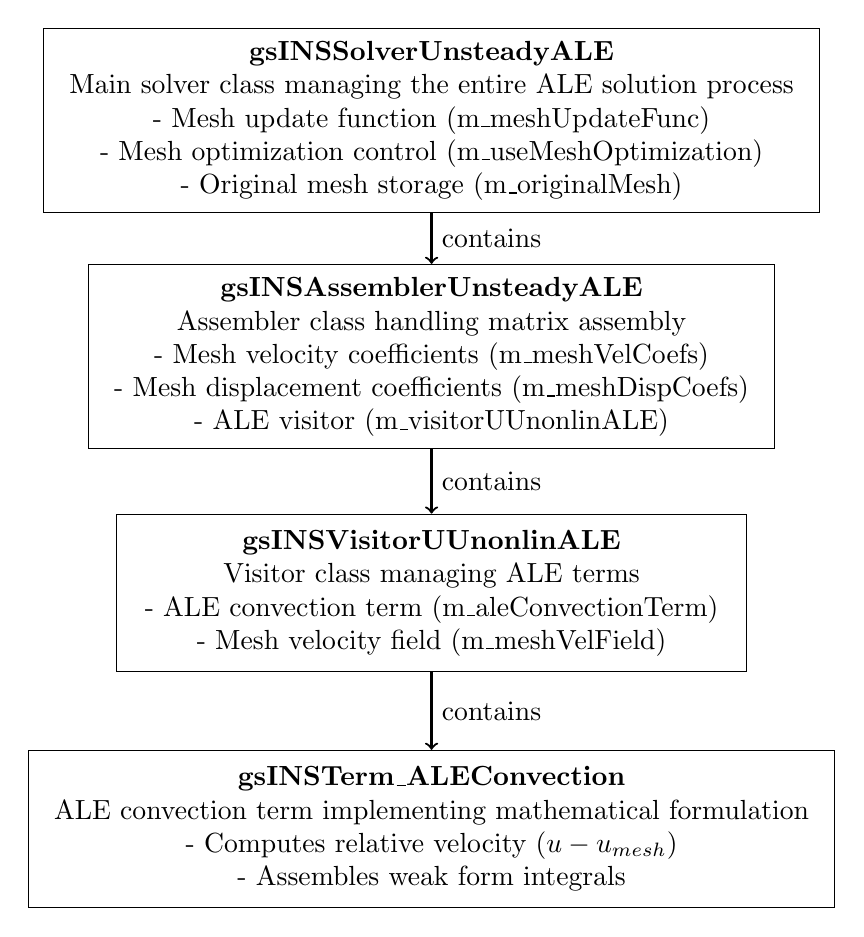
\begin{tikzpicture}[
    class/.style={rectangle, draw, minimum width=8cm, minimum height=2cm, text centered},
    arrow/.style={->, thick}
]
    % Class nodes
    \node[class] (solver) at (0,0) {
        \begin{tabular}{c}
        \textbf{gsINSSolverUnsteadyALE}\\
        Main solver class managing the entire ALE solution process\\
        - Mesh update function (m\_meshUpdateFunc)\\
        - Mesh optimization control (m\_useMeshOptimization)\\
        - Original mesh storage (m\_originalMesh)
        \end{tabular}
    };
    
    \node[class] (assembler) at (0,-3) {
        \begin{tabular}{c}
        \textbf{gsINSAssemblerUnsteadyALE}\\
        Assembler class handling matrix assembly\\
        - Mesh velocity coefficients (m\_meshVelCoefs)\\
        - Mesh displacement coefficients (m\_meshDispCoefs)\\
        - ALE visitor (m\_visitorUUnonlinALE)
        \end{tabular}
    };
    
    \node[class] (visitor) at (0,-6) {
        \begin{tabular}{c}
        \textbf{gsINSVisitorUUnonlinALE}\\
        Visitor class managing ALE terms\\
        - ALE convection term (m\_aleConvectionTerm)\\
        - Mesh velocity field (m\_meshVelField)
        \end{tabular}
    };
    
    \node[class] (term) at (0,-9) {
        \begin{tabular}{c}
        \textbf{gsINSTerm\_ALEConvection}\\
        ALE convection term implementing mathematical formulation\\
        - Computes relative velocity $(u - u_{mesh})$\\
        - Assembles weak form integrals
        \end{tabular}
    };
    
    % Arrows
    \draw[arrow] (solver) -- node[right] {contains} (assembler);
    \draw[arrow] (assembler) -- node[right] {contains} (visitor);
    \draw[arrow] (visitor) -- node[right] {contains} (term);
\end{tikzpicture}
\caption{ALE implementation class hierarchy}
\end{figure}

\section{gsINSTermsALE.h}
\label{sec:gsINSTermsALE}

\subsection{Overview}
Defines the weak form implementation of ALE convection terms, which is the core mathematical expression of the ALE method.

\subsection{Main Class: gsINSTerm\_ALEConvection}

\subsubsection{Class Definition (Lines 21-22)}

\begin{lstlisting}
template <class T>
class gsINSTerm_ALEConvection : public gsFlowTermNonlin<T>
\end{lstlisting}

\subsubsection{Core Functionality}
\begin{itemize}
    \item \textbf{ALE convection term}: Implements the weak form of $((u - u_{mesh}) \cdot \nabla\varphi_{trial}) * \varphi_{test}$ (Line 18)
    \item \textbf{Relative velocity computation}: $u_{rel} = u - u_{mesh}$ (Line 96)
    \item \textbf{Physical space gradient transformation}: Transforms parametric space gradients to physical space (Line 119)
\end{itemize}

\subsubsection{Key Member Variables (Lines 30-36)}
\begin{itemize}
    \item \texttt{m\_tarDim}: Target dimension (typically 2 or 3)
    \item \texttt{m\_meshVelVals}: Mesh velocity values at quadrature points
    \item \texttt{m\_meshVelField}: Mesh velocity field pointer
\end{itemize}

\subsubsection{Core Methods}

\paragraph{\texttt{computeMeshVelocity()} (Lines 57-70)}

\begin{lstlisting}
void computeMeshVelocity(const gsMapData<T>& mapData)
\end{lstlisting}
\begin{itemize}
    \item Computes mesh velocity at quadrature points
    \item Defaults to zero if mesh velocity field is not set (Line 68)
\end{itemize}

\paragraph{\texttt{assemble()} (Lines 78-134)}

\begin{lstlisting}
virtual void assemble(const gsMapData<T>& mapData, 
                     const gsVector<T>& quWeights, 
                     const std::vector<gsMatrix<T>>& testFunData, 
                     const std::vector<gsMatrix<T>>& trialFunData, 
                     gsMatrix<T>& localMat)
\end{lstlisting}
\begin{itemize}
    \item Assembles local matrix for ALE convection term
    \item Computes relative velocity \texttt{relativeVel = m\_solUVals - m\_meshVelVals} (Line 96)
    \item Computes gradients in physical space (Line 119)
    \item Integrates $\int (\varphi_{test} \cdot ((u-w)\cdot\nabla\varphi_{trial})) d\Omega$ (Lines 131-132)
\end{itemize}

\subsubsection{Design Features}
\begin{itemize}
    \item \textbf{Flexibility}: Supports dynamic mesh velocity field setting
    \item \textbf{Efficiency}: Computes mesh velocity only when needed
    \item \textbf{Generality}: Supports both 2D and 3D problems
\end{itemize}

\section{gsINSVisitorsALE.h}
\label{sec:gsINSVisitorsALE}

\subsection{Overview}
Provides ALE visitor classes that manage ALE convection terms and integrate them into the assembly process.

\subsection{Main Class: gsINSVisitorUUnonlinALE}

\subsubsection{Class Definition (Lines 22-24)}

\begin{lstlisting}
template <class T, int MatOrder = RowMajor>
class gsINSVisitorUUnonlinALE : public gsINSVisitorUU<T, MatOrder>
\end{lstlisting}

\subsubsection{Core Functionality}
\begin{itemize}
    \item \textbf{ALE term management}: Creates and manages \texttt{gsINSTerm\_ALEConvection} instances
    \item \textbf{Interface adaptation}: Connects ALE terms with standard INS assembly framework
    \item \textbf{State management}: Updates mesh velocity fields and current solutions
\end{itemize}

\subsubsection{Constructors}
Two construction methods are provided:

\paragraph{Recommended Method (with paramsPtr) (Lines 43-58)}

\begin{lstlisting}
gsINSVisitorUUnonlinALE(typename gsFlowSolverParams<T>::Ptr paramsPtr,
                       const std::vector<gsDofMapper>& dofMappers,
                       index_t targetDim = 2,
                       const gsField<T>* meshVelField = nullptr)
\end{lstlisting}

\paragraph{Compatibility Method (without paramsPtr) (Lines 61-75)}

\begin{lstlisting}
gsINSVisitorUUnonlinALE(const std::vector<gsDofMapper>& dofMappers,
                       index_t targetDim = 2,
                       const gsField<T>* meshVelField = nullptr)
\end{lstlisting}

\subsubsection{Key Methods}

\paragraph{\texttt{setMeshVelocityField()} (Lines 83-89)}

\begin{lstlisting}
void setMeshVelocityField(const gsField<T>* meshVelField)
\end{lstlisting}
\begin{itemize}
    \item Updates mesh velocity field
    \item Synchronously updates internal ALE convection term (Line 88)
\end{itemize}

\paragraph{\texttt{setCurrentSolution()} (Lines 92-100)}

\begin{lstlisting}
void setCurrentSolution(const gsField<T>& solution)
\end{lstlisting}
\begin{itemize}
    \item Sets current velocity solution
    \item Passes to all nonlinear terms
\end{itemize}

\section{gsINSAssemblerALE.h}
\label{sec:gsINSAssemblerALE}

\subsection{Overview}
Extends the unsteady INS assembler with ALE functionality, handling mesh motion and velocity computation.

\subsection{Main Class: gsINSAssemblerUnsteadyALE}

\subsubsection{Class Definition (Lines 21-23)}

\begin{lstlisting}
template <class T, int MatOrder = RowMajor>
class gsINSAssemblerUnsteadyALE : public gsINSAssemblerUnsteady<T, MatOrder>
\end{lstlisting}

\subsubsection{Key Member Variables (Lines 39-51)}

\begin{lstlisting}
gsMatrix<T> m_meshVelCoefs;      // Mesh velocity coefficients (Line 40)
gsMatrix<T> m_meshDispCoefs;     // Current mesh displacement (Line 41)
gsMatrix<T> m_meshDispOld;       // Previous time step mesh displacement (Line 42)
gsINSVisitorUUnonlinALE<T, MatOrder>* m_visitorUUnonlinALE;  // ALE visitor (Line 45)
bool m_isALEActive;              // ALE activation flag (Line 48)
gsField<T>* m_tempMeshVelField;  // Temporary mesh velocity field (Line 51)
\end{lstlisting}

\subsubsection{Core Methods}

\paragraph{\texttt{initialize()} (Lines 70-86)}

\begin{lstlisting}
virtual void initialize() override
\end{lstlisting}
\begin{itemize}
    \item Initializes base class (Line 73)
    \item Allocates mesh coefficient storage space (Lines 76-79)
    \item Creates ALE visitor (Lines 82-83)
\end{itemize}

\paragraph{\texttt{updateMesh()} (Lines 108-131)}

\begin{lstlisting}
void updateMesh(const gsMatrix<T>& meshDispNew)
\end{lstlisting}
\begin{itemize}
    \item Computes mesh velocity: $v_{mesh} = (disp_{new} - disp_{old}) / dt$ (Line 123)
    \item Updates displacement storage (Line 130)
    \item Extends vectors to full size (includes zero pressure part) (Lines 121-127)
\end{itemize}

\paragraph{\texttt{assembleNonlinearPart()} (Lines 154-195)}

\begin{lstlisting}
virtual void assembleNonlinearPart() override
\end{lstlisting}
\begin{itemize}
    \item Uses ALE visitor if ALE is active (Line 156)
    \item Creates temporary mesh velocity field (Lines 159-160)
    \item Assembles ALE convection terms (Lines 181, 187)
\end{itemize}

\section{gsINSSolverALE.h}
\label{sec:gsINSSolverALE}

\subsection{Overview}
Top-level ALE solver class providing complete ALE flow solution functionality, including mesh optimization and FSI coupling support.

\subsection{Main Class: gsINSSolverUnsteadyALE}

\subsubsection{Class Definition (Lines 24-26)}

\begin{lstlisting}
template <class T = real_t, int MatOrder = RowMajor>
class gsINSSolverUnsteadyALE : public gsINSSolverUnsteady<T, MatOrder>
\end{lstlisting}

\subsubsection{Key Member Variables (Lines 38-61)}

\begin{lstlisting}
bool m_isALEActive;                          // ALE activation flag (Line 38)
std::function<gsMatrix<T>(T)> m_meshUpdateFunc;  // Mesh update function (Line 41)
bool m_useMeshOptimization;                  // Mesh optimization flag (Line 44)
bool m_useDynamicBoundaryMapping;            // Dynamic boundary mapping flag (Line 47)
gsMultiPatch<T> m_originalMesh;              // Original mesh (Line 53)
gsMatrix<T> m_previousDisp;                  // Previous time step displacement (Line 56)
T m_rotationPeriod;                          // Rotation period (Line 59)
gsVector<T> m_rotationCenter;                // Rotation center (Line 60)
\end{lstlisting}

\subsubsection{Core Methods}

\paragraph{\texttt{setALEActive()} (Lines 87-99)}

\begin{lstlisting}
void setALEActive(bool active)
\end{lstlisting}
\begin{itemize}
    \item Activates/deactivates ALE (Line 91)
    \item Stores original mesh on first activation (Line 96)
    \item Synchronously updates assembler state (Line 91)
\end{itemize}

\paragraph{\texttt{nextIteration()} (Lines 183-200)}

\begin{lstlisting}
virtual void nextIteration() override
\end{lstlisting}
Main ALE time stepping function with the following sequence:
\begin{enumerate}
    \item Apply mesh displacement (Line 189)
    \item Mesh optimization (optional) (Line 194)
    \item Solve flow problem (Line 199)
\end{enumerate}

\paragraph{\texttt{optimizeMesh()} (Lines 247-290)}

\begin{lstlisting}
void optimizeMesh()
\end{lstlisting}
\begin{itemize}
    \item Uses gsBarrierPatch to optimize mesh quality (Line 275)
    \item Supports standard and dynamic boundary mapping modes (Line 254)
    \item Exception handling: continues computation if optimization fails (Lines 286-289)
\end{itemize}

\subsection{Helper Class: gsFSIHelper (Lines 296-387)}

Provides utility functions for fluid-structure interaction (framework reserved for future implementation).

\subsubsection{Static Utility Methods (Lines 365-370)}
\begin{lstlisting}
static gsMatrix<T> computeMeshVelocity(const gsMatrix<T>& dispNew,
                                      const gsMatrix<T>& dispOld,
                                      T dt)
\end{lstlisting}
\begin{itemize}
    \item Computes mesh velocity from displacement history
    \item Uses backward difference scheme (Line 369)
\end{itemize}

\section{Class Hierarchy}
\label{sec:class-hierarchy}

\subsection{Inheritance Relationships}

\begin{verbatim}
gsFlowTermNonlin<T>
    |-- gsINSTerm_ALEConvection<T>

gsINSVisitorUU<T, MatOrder>
    |-- gsINSVisitorUUnonlinALE<T, MatOrder>

gsINSAssemblerUnsteady<T, MatOrder>
    |-- gsINSAssemblerUnsteadyALE<T, MatOrder>

gsINSSolverUnsteady<T, MatOrder>
    |-- gsINSSolverUnsteadyALE<T, MatOrder>

Independent helper class:
    gsFSIHelper<T>
\end{verbatim}

\subsection{Detailed Class Structure}

The following sections provide detailed UML-style descriptions of each class:

\subsubsection{\texttt{gsINSTerm\_ALEConvection<T>}}

\begin{itemize}
    \item \textbf{Private Members:}
    \begin{itemize}
        \item \texttt{m\_tarDim: index\_t} -- Target dimension
        \item \texttt{m\_meshVelVals: gsMatrix<T>} -- Mesh velocity values
        \item \texttt{m\_meshVelField: const gsField<T>*} -- Mesh velocity field pointer
    \end{itemize}
    \item \textbf{Public Methods:}
    \begin{itemize}
        \item \texttt{setMeshVelocityField(field): void}
        \item \texttt{computeMeshVelocity(mapData): void}
        \item \texttt{assemble(...): void override}
    \end{itemize}
\end{itemize}

\subsubsection{\texttt{gsINSVisitorUUnonlinALE<T, MatOrder>}}

\begin{itemize}
    \item \textbf{Private Members:}
    \begin{itemize}
        \item \texttt{m\_tarDim: index\_t} -- Target dimension
        \item \texttt{m\_meshVelField: const gsField<T>*} -- Mesh velocity field
        \item \texttt{m\_aleConvectionTerm: gsINSTerm\_ALEConvection<T>*} -- ALE term
    \end{itemize}
    \item \textbf{Public Methods:}
    \begin{itemize}
        \item \texttt{setMeshVelocityField(field): void}
        \item \texttt{setCurrentSolution(solution): void}
    \end{itemize}
\end{itemize}

\subsubsection{\texttt{gsINSAssemblerUnsteadyALE<T, MatOrder>}}

\begin{itemize}
    \item \textbf{Private Members:}
    \begin{itemize}
        \item \texttt{m\_meshVelCoefs: gsMatrix<T>} -- Mesh velocity coefficients
        \item \texttt{m\_meshDispCoefs: gsMatrix<T>} -- Mesh displacement coefficients
        \item \texttt{m\_meshDispOld: gsMatrix<T>} -- Previous mesh displacement
        \item \texttt{m\_visitorUUnonlinALE: gsINSVisitorUUnonlinALE<T>*} -- ALE visitor
        \item \texttt{m\_isALEActive: bool} -- ALE activation flag
        \item \texttt{m\_tempMeshVelField: gsField<T>*} -- Temporary mesh velocity field
    \end{itemize}
    \item \textbf{Public Methods:}
    \begin{itemize}
        \item \texttt{initialize(): void override}
        \item \texttt{updateMesh(meshDispNew): void}
        \item \texttt{assembleNonlinearPart(): void override}
        \item \texttt{getMeshVelocityField(): gsField<T>}
        \item \texttt{getMeshDisplacementField(): gsField<T>}
    \end{itemize}
\end{itemize}

\subsubsection{\texttt{gsINSSolverUnsteadyALE<T, MatOrder>}}

\begin{itemize}
    \item \textbf{Private Members:}
    \begin{itemize}
        \item \texttt{m\_isALEActive: bool} -- ALE activation flag
        \item \texttt{m\_meshUpdateFunc: std::function<gsMatrix<T>(T)>} -- Mesh update function
        \item \texttt{m\_useMeshOptimization: bool} -- Mesh optimization flag
        \item \texttt{m\_originalMesh: gsMultiPatch<T>} -- Original mesh
        \item \texttt{m\_previousDisp: gsMatrix<T>} -- Previous displacement
    \end{itemize}
    \item \textbf{Public Methods:}
    \begin{itemize}
        \item \texttt{setALEActive(active): void}
        \item \texttt{setMeshUpdateFunction(func): void}
        \item \texttt{nextIteration(): void override}
        \item \texttt{optimizeMesh(): void}
        \item \texttt{setMeshOptimization(enable): void}
    \end{itemize}
\end{itemize}

\section{Usage Flow}
\label{sec:usage-flow}

\subsection{Basic Usage Steps}

\begin{enumerate}
    \item \textbf{Create solver}
    
    \begin{lstlisting}
gsINSSolverUnsteadyALE<> solver(paramsPtr);
solver.initialize();
    \end{lstlisting}
    
    \item \textbf{Activate ALE}
    
    \begin{lstlisting}
solver.setALEActive(true);
    \end{lstlisting}
    
    \item \textbf{Set mesh motion}
    
    \begin{lstlisting}
solver.setMeshUpdateFunction([](real_t t) {
    return computeDisplacement(t);
});
    \end{lstlisting}
    
    \item \textbf{Optional: Enable mesh optimization}
    
    \begin{lstlisting}
solver.setMeshOptimization(true);
solver.getMeshOptOptions().setInt("Verbose", 1);
    \end{lstlisting}
    
    \item \textbf{Time stepping}
    
    \begin{lstlisting}
for (int step = 0; step < nSteps; ++step) {
    solver.nextIteration();
}
    \end{lstlisting}
\end{enumerate}

\subsection{Data Flow}

\begin{verbatim}
User-defined mesh motion
    |
    v
gsINSSolverUnsteadyALE::nextIteration()
    |
    v
applyMeshDisplacement()
    |
    v
gsINSAssemblerUnsteadyALE::updateMesh()
    |
    v
gsINSAssemblerUnsteadyALE::assembleNonlinearPart()
    |
    v
gsINSVisitorUUnonlinALE (with mesh velocity)
    |
    v
gsINSTerm_ALEConvection::assemble()
    |
    v
Assemble ALE convection term matrix
\end{verbatim}

\subsection{Key Design Decisions}

\begin{enumerate}
    \item \textbf{Minimal invasiveness}: Extension through inheritance rather than base class modification
    \item \textbf{Flexibility}: Support for dynamic switching between ALE/standard modes
    \item \textbf{Efficiency}: Additional data structures created only when needed
    \item \textbf{Extensibility}: Reserved interfaces for FSI and other coupling methods
    \item \textbf{Robustness}: Fault tolerance when mesh optimization fails
\end{enumerate}

\section{Mesh Optimization with Barrier Functions}

\subsection{Overview}
The ALE implementation integrates barrier function-based mesh optimization to maintain mesh quality during large deformations. This is particularly important for FSI simulations where the mesh can undergo significant distortion.

\subsection{Key Components}

\subsubsection{gsBarrierPatch Integration}
The \texttt{gsINSSolverUnsteadyALE} class integrates with G+Smo's \texttt{gsBarrierPatch} for mesh optimization:

\begin{lstlisting}
// In gsINSSolverUnsteadyALE.h
#include <gsModeling/gsBarrierPatch.h>
#include <gsIncompressibleFlow/src/gsBarrierPatchDynamic.h>
\end{lstlisting}

\subsubsection{Mesh Optimization Method}
The \texttt{optimizeMesh()} method (Lines 247-290) implements the barrier function optimization:

\begin{lstlisting}
void optimizeMesh()
{
    // Get current mesh from assembler
    gsMultiPatch<T>& patches = const_cast<gsMultiPatch<T>&>(
        m_assemblerPtr->getPatches());
    
    if (m_useDynamicBoundaryMapping && m_meshUpdateFunc)
    {
        // Apply gsBarrierPatchDynamic for rotating domains
        gsBarrierPatchDynamic<2, T> opt;
        opt.setDynamicBoundaryMapping(true);
        opt.setRotationAngle(getCurrentRotationAngle());
        opt.setRotationCenter(m_rotationCenter);
        patches = opt.compute(patches, m_meshOptOptions);
    }
    else
    {
        // Use standard gsBarrierPatch
        gsBarrierPatch<2, T> opt(patches, false);
        opt.options() = m_meshOptOptions;
        opt.compute();
        patches = opt.result();
    }
}
\end{lstlisting}

\subsection{Barrier Function Formulation}
The barrier function approach prevents mesh inversion by minimizing an objective function:

\begin{equation}
\min_{\mathbf{x}} \sum_{e} \int_{\Omega_e} \mu(J_e) \, d\Omega
\end{equation}

where $\mu(J)$ is a barrier function that approaches infinity as the Jacobian $J \to 0$:

\begin{equation}
\mu(J) = \frac{1}{2} \left( J + \frac{1}{J} \right) - 1
\end{equation}

\subsection{Configuration Options}
The mesh optimization can be configured through \texttt{m\_meshOptOptions}:

\begin{lstlisting}
// Initialize mesh optimization options
m_meshOptOptions.addInt("Verbose", "Verbosity level", 0);
m_meshOptOptions.addInt("ParamMethod", "Parametrization method", 1);
m_meshOptOptions.addInt("AAPreconditionType", "AA precondition type", 0);
\end{lstlisting}

\subsection{Usage Example}

\begin{lstlisting}
// Enable mesh optimization
solver.setMeshOptimization(true);

// Configure optimization parameters
solver.getMeshOptOptions().setInt("Verbose", 1);
solver.getMeshOptOptions().setInt("ParamMethod", 1);

// For rotating domains
solver.setDynamicBoundaryMapping(true);
solver.setRotationParameters(period, center);
\end{lstlisting}

\subsection{Dynamic Boundary Mapping}
For rotating machinery applications, the \texttt{gsBarrierPatchDynamic} extension provides:

\begin{itemize}
    \item Automatic detection of approaching boundaries
    \item Dynamic remapping of boundary nodes
    \item Preservation of mesh topology during rotation
    \item Prevention of mesh tangling at sliding interfaces
\end{itemize}

\subsection{Error Handling}
The implementation includes robust error handling:

\begin{lstlisting}
try {
    // Mesh optimization code
    patches = opt.compute(patches, m_meshOptOptions);
}
catch (const std::exception& e) {
    gsWarn << "Mesh optimization failed: " << e.what() << "\n";
    gsWarn << "Continuing with unoptimized mesh.\n";
}
\end{lstlisting}

This ensures that the simulation continues even if mesh optimization fails, improving robustness for production use.

\section{Summary}

This ALE implementation provides a complete, efficient, and flexible moving mesh flow solution framework. Through a layered design from low-level weak form terms to high-level solvers, each layer has clear responsibilities and interfaces. The integration of barrier function-based mesh optimization ensures mesh quality is maintained throughout the simulation, making it particularly suitable for handling complex flow problems involving moving boundaries such as fluid-structure interaction and rotating machinery.

\end{document}